\documentclass[10pt,twocolumn]{article}

% use the oxycomps style file
\usepackage{oxycomps}
\usepackage{pgfplots}
\pgfplotsset{compat=1.17}


% usage: \fixme[comments describing issue]{text to be fixed}
% define \fixme as not doing anything special
\newcommand{\fixme}[2][]{#2}
% overwrite it so it shows up as red
\renewcommand{\fixme}[2][]{\textcolor{red}{#2}}
% overwrite it again so related text shows as footnotes
%\renewcommand{\fixme}[2][]{\textcolor{red}{#2\footnote{#1}}}

% read references.bib for the bibtex data
\bibliography{references}

% include metadata in the generated pdf file
\pdfinfo{
    /Title (The Occidental Computer Science Comprehensive Project: Goals, Timeline, Format, and Advice)
    /Author (Ruige Wu)
}

% set the title and author information
\title{Fusing Elements and Strategy: \\Creating Depth in 2D Top-Down RPG Gameplay}
\author{Ruige Wu}
\affiliation{Occidental College}
\email{wur@oxy.edu}

\begin{document}

\maketitle

\section{Problem Statement}
In traditional 2D Top Down RPGs, players often encounter a significant limitation in combat skill management due to the constraints of keyboard input. Players typically possess a wide array of skills gained through leveling up; however, they can only access a limited set, usually six, at any given time due to the physical limitations of keyboard controls. This restriction is particularly problematic during intense real-time combat scenarios where quick decision-making is crucial. The necessity for keybindings tied to movement (WASD), dodging (Shift), and other actions further compounds this issue, leading to an overloaded left hand that must also aim simultaneously.
This situation raises two critical challenges: first, it restricts player agency by limiting their ability to dynamically adapt their skill set based on immediate combat needs; second, it risks frustrating gameplay experiences as players may struggle with intricate key combinations under pressure. Traditional solutions like time-stop skill selection detract from immersion and disrupt the fast-paced nature of real-time combat.
Addressing these issues is vital for enhancing player engagement and satisfaction within 2D Top Down RPGs. By creating an innovative spell-casting system that reduces reliance on multiple key inputs while allowing for extensive skill customization in real-time scenarios, my project aims to empower players with greater flexibility and responsiveness in gameplay.
The importance of this problem extends beyond individual enjoyment; it reflects broader trends in game design emphasizing accessibility and user experience. As gaming continues to evolve into a primary form of entertainment across diverse demographics, including those who may struggle with complex input methods the need for intuitive controls becomes increasingly significant. By developing an effective solution within my Comps project, I hope not only to improve individual player experiences but also contribute valuable insights into accessible game design principles that can benefit the wider gaming community.

\section{Technical Background}

To fully grasp the problem addressed in this project and the solutions implemented, it is essential to understand several foundational concepts related to game development, real-time combat systems, and algorithmic elements such as pathfinding and dynamic user interaction. This section provides an overview of the key technical components and terms utilized throughout the project.

\subsection{2D Top-Down RPGs}
A 2D Top-Down RPG (Role-Playing Game) is a game genre where the player views the world from a bird's-eye perspective, controlling a character as they explore environments, engage in combat, and interact with the game world. The real-time combat system in such games poses unique challenges:
\begin{itemize}
    \item \textbf{Dynamic Movement and Combat}: Players must simultaneously manage movement, targeting, and attacks, creating high input demand.
    \item \textbf{Limited Keybindings}: The need to balance movement controls (e.g., WASD) with a diverse set of combat abilities is constrained by the finite number of keys within reach of the player.
    \item \textbf{Strategic Depth}: Designing systems that encourage thoughtful decisions without overwhelming players is critical to enhancing gameplay satisfaction.
\end{itemize}

This project tackles these challenges by developing an innovative spell-casting system that uses elemental combinations instead of traditional keybindings, allowing for both variety and simplicity.

\subsection{Elemental Systems and Wu Xing}
The elemental system implemented in this project is inspired by Wu Xing, a traditional Chinese philosophical framework that defines interactions between five elements: Metal, Wood, Water, Fire, and Earth. Wu Xing is often used in games to model relationships between elements, providing both thematic depth and gameplay mechanics.

\begin{itemize}
    \item \textbf{Elemental Relationships}:
        \begin{itemize}
            \item \textbf{Generative Cycle (Mutual Generation)}: Elements can reinforce one another, such as Water nurturing Wood.
            \item \textbf{Overcoming Cycle (Mutual Overcoming)}: Elements can counteract one another, such as Fire overcoming Metal.
        \end{itemize}
    \item \textbf{In-Game Application}:
        \begin{itemize}
            \item The primary element of a player's spell interacts with the current area's element to amplify or reduce its effectiveness.
            \item Spells aligned with the area’s element are amplified by 25\%, while opposing elements result in a 25\% reduction in damage.
        \end{itemize}
\end{itemize}

These interactions encourage players to adapt their strategies based on the environment, adding a dynamic layer of strategy to combat.

\subsection{Pathfinding with A* Algorithm}
Pathfinding is a critical component of the enemy AI, enabling enemies to navigate the game world and chase the player effectively. The project leverages the A* (A-Star) algorithm, a widely used search algorithm in game development for finding the shortest path between two points.

\subsubsection{How A* Works}
The A* algorithm combines two heuristics to determine the optimal path:
\begin{itemize}
    \item \textbf{g(n)}: The cost of reaching node \(n\) from the start node.
    \item \textbf{h(n)}: The estimated cost from node \(n\) to the goal (heuristic function).
    \item \textbf{f(n)}: The total estimated cost, calculated as \(f(n) = g(n) + h(n)\).
\end{itemize}

By prioritizing nodes with the lowest \(f(n)\) value, A* ensures efficient pathfinding. In this project, the A* Pathfinding plugin by Aron Granberg is used to implement this algorithm, with the following customizations:
\begin{itemize}
    \item \textbf{Dynamic Graph Updates}: When the player moves between areas, the A* grid graph is re-scanned to account for new obstacles and enemy placements.
    \item \textbf{Seeker and AIPath Components}: These components calculate paths and control enemy movement along the paths, ensuring smooth and realistic navigation.
\end{itemize}

\subsection{Spell-Casting System: Orb-Based Selection}
The spell-casting system introduces a novel approach to skill management by leveraging a cycling orb interface for element selection. Key concepts include:
\begin{itemize}
    \item \textbf{Highlighting Mechanism}:
        \begin{itemize}
            \item Five elemental orbs are displayed, cycling through a highlight state.
            \item Players press a key (Space) to select the currently highlighted orb.
        \end{itemize}
    \item \textbf{Elemental Combinations}:
        \begin{itemize}
            \item Players can select up to three elements per spell, with each combination mapped to a specific spell in the \texttt{SpellBook}.
            \item The order of selected elements is significant, as it determines the resulting spell's attributes.
        \end{itemize}
    \item \textbf{Interaction with \texttt{SpellBook}}:
        \begin{itemize}
            \item The \texttt{SpellBook} stores pre-defined spells, each with a unique key representing its elemental combination.
            \item When a spell is cast, its prefab is instantiated, and its effects (e.g., damage, area of effect) are applied in-game.
        \end{itemize}
\end{itemize}

\subsection{UI and Player Feedback}
User interface design is critical for conveying real-time information to the player. The following elements are integrated into the game:
\begin{itemize}
    \item \textbf{Health Bar}: Visually represents the player’s current health, providing immediate feedback on damage taken.
    \item \textbf{Timer Indicators}: Show the remaining time for the exit portal to unlock and the player's total survival time.
    \item \textbf{Elemental Zone Indicator}: Displays the current area’s elemental property, helping players adapt their strategies.
\end{itemize}

Dynamic updates to these UI elements are managed by the \texttt{UIManager}, which listens for game events such as damage taken or portal activation.

\subsection{Game Object and Script Interactions}
The project’s modular architecture ensures that game objects and scripts work cohesively while remaining easy to extend:
\begin{itemize}
    \item \textbf{GameManager} initializes the game state and activates the starting area.
    \item \textbf{PortalSystem} handles area transitions, including activating and deactivating areas and resetting the A* graph.
    \item \textbf{EnemySpawner} dynamically spawns enemies in active areas, ensuring a consistent challenge.
    \item \textbf{SpellBook} stores all spells and serves as a lookup table for the \texttt{ElementSelector} when casting spells.
    \item \textbf{AreaManager} tracks the environmental element and manages area-specific interactions, such as amplifying or weakening spells.
\end{itemize}

\subsection{Iterative Design and Testing}
The project underwent multiple iterations to refine its mechanics and balance:
\begin{itemize}
    \item Initial designs relied on complex keybindings, which were replaced by the orb-based selection system to improve accessibility and reduce cognitive load.
    \item Testing revealed the optimal highlight interval for the orbs (0.5 seconds), balancing speed and accuracy.
    \item Environmental interactions were fine-tuned to ensure they were intuitive and impactful without overwhelming players.
\end{itemize}

\subsection{Conclusion}
This technical background outlines the foundational concepts and systems that underpin the project, providing the necessary context for understanding the design choices and their implementation. By combining elemental mechanics, pathfinding algorithms, and innovative UI designs, the project offers a scalable and immersive solution to the challenges of real-time combat in 2D Top-Down RPGs.

\section{Prior Work}
My design draws inspiration from a diverse array of games, each contributing unique mechanics and thematic elements that inform my approach to developing a real-time combat system in a 2D Top Down RPG. The key titles that have influenced my work include MiChangSheng, Magic: The Gathering, Sorcery!, and The Legend of Zelda: Tears of the Kingdom.

\subsection{MiChangSheng}
MiChangSheng, a turn-based game rooted in traditional Chinese culture, employs an elemental system where players combine different elements to unleash skills and summon followers. Its use of the five elements (Wood, Fire, Earth, Metal, Water) as foundational components for skill interaction serves as an innovative model for my own spell-casting system. By adapting this concept into my real-time combat framework, I enable players to select from these elemental categories through intuitive keystrokes—effectively allowing for rapid combinations that yield dozens or even hundreds of unique spells with minimal input.

\subsection{Magic: The Gathering}
As one of the most popular collectible card games (CCGs), Magic: The Gathering introduces strategic depth through its combination mechanics involving various card types and colors (representing different mana). This game's emphasis on resource management and tactical combinations resonates with my vision for skill selection within an RPG context. Drawing from its principles allows me to create gameplay that rewards thoughtful planning and adaptability in combat scenarios—transforming player interactions into more than mere button mashing by fostering strategic spell choice based on real-time needs.

\subsection{Sorcery!}
Sorcery!, known for its visual novel style combined with interactive storytelling mechanisms based on player choices, offers significant insight into how unexpected outcomes can arise from spell combinations. Unlike traditional designs where success is often guaranteed with specific spells or combos, Sorcery! highlights that some combinations may lead to failure or unforeseen consequences. This notion aligns closely with the principles of mutual generation and overcoming found within Chinese philosophy regarding elemental interactions—where certain elements may not synergize effectively when combined due to their inherent antagonisms (e.g., Metal overcomes Wood). Incorporating this understanding into my game encourages players not only to experiment but also strategically consider which spells they choose based on their elemental properties—a layer enriching both challenge and engagement.

\subsection{The Legend of Zelda: Tears of the Kingdom}
Finally, Tears of the Kingdom exemplifies modern advancements in environmental interaction through intuitive gameplay mechanics where elemental powers influence surroundings creatively, from manipulating terrain to interacting with weather patterns. This has profoundly shaped my design philosophy; thus integrating similar synergies between spells cast by players in my game has become essential, not just as tools against foes but also as mechanisms impacting environmental dynamics further enhancing immersive experiences.

\subsection{Conclusion}
By synthesizing insights drawn from these influential works where each emphasizing unique aspects such as elemental mastery (MiChangSheng), strategic resource management (Magic: The Gathering), unexpected outcomes from decisions made during gameplay (*Sorcery!*), and environmental interactivity (*Tears of the Kingdom*). My project seeks to innovate within established frameworks while offering new solutions tailored towards improving user experience during real-time gameplay sessions.
In conclusion, this thematic discussion highlights how these varied influences converge within my project’s design philosophy, aiming not only at enhancing individual agency during combat but also enriching overall engagement through integrated systems that reward creativity across multiple dimensions.

\section{Methods}

\subsection{Overview}
To address the challenge of managing diverse combat skills within a real-time 2D top-down RPG, this project implemented a novel spell-casting system based on elemental combinations. The system leverages intuitive input mechanics, allowing players to dynamically select and execute spells by combining elemental inputs in sequence. Supporting systems, including enemy AI, environmental interactions, and area management, were developed to enhance the player's combat experience and integrate the spell system into a cohesive game environment.

\subsection{Spell System Design}
The spell-casting system is the centerpiece of this project, directly addressing the problem of skill management in real-time combat by reducing reliance on numerous keybindings while maintaining versatility and strategic depth.

\subsubsection{Mechanics of the Spell-Casting System}
The system employs five elemental orbs, each representing one of the five elements: Metal, Wood, Water, Fire, and Earth. These orbs cycle through a highlighting sequence, allowing players to select an element by pressing a single key (Space) when the desired orb is highlighted. This streamlined interaction eliminat\textbf{}es the need for extensive keybindings, freeing players to focus on combat and strategy.

Players can select a maximum of three elements for each spell. The first chosen element becomes the primary element, defining the spell's interaction with the environment. The second and third elements, known as secondary elements, expand the variety of spells but are constrained by elemental compatibility rules. For instance, secondary elements cannot be mutually restraining (e.g., Fire and Water cannot coexist in the same spell). This system ensures that spells remain balanced and strategic, encouraging experimentation while maintaining intuitive gameplay.

\begin{figure}[h]
    \centering
    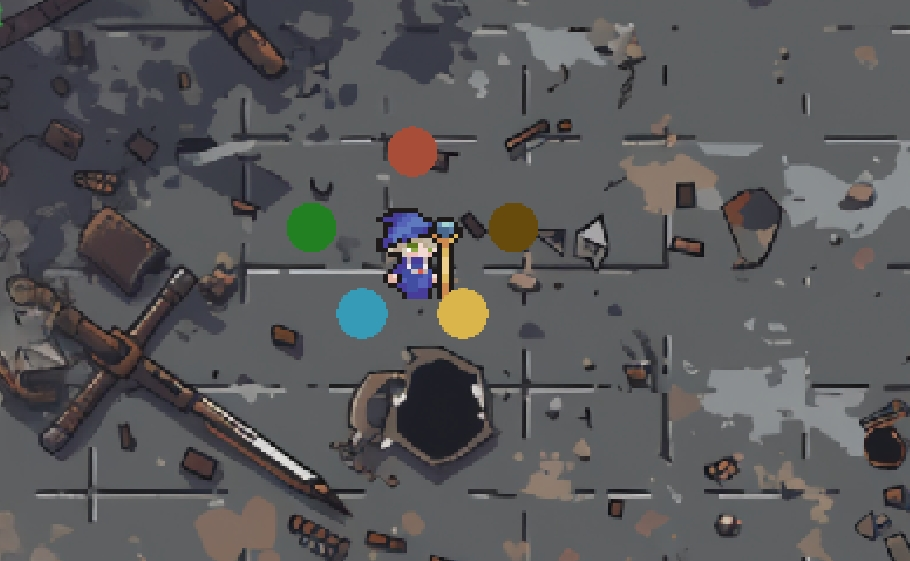
\includegraphics[width=\columnwidth]{figure1.png} % Use the name of your image file
    \caption{Spell Casting System}
    \label{fig:figure1} % Reference label for the image
\end{figure}


\subsubsection{Integration of Elemental Combinations}
Elemental combinations are programmed to produce diverse spell effects, with each combination assigned unique attributes such as damage, area of effect, or duration. A modular design was used to store elemental combinations and their effects in a SpellBook Manager, allowing easy scalability. Players are dynamically prompted to cast their spell once three elements have been chosen, ensuring a smooth transition from selection to execution.

\subsection{Game Environment and Interactions}

\subsubsection{Elemental Zones}
Each area of the map is assigned an elemental property (e.g., Fire, Water). The primary element of the player's spell interacts with the environment based on Wu Xing principles. For example:
\begin{itemize}
    \item When the primary element aligns with the environment (e.g., Fire spell in a Fire zone), the spell's power is amplified by 25 percents.
    \item If the environment restrains the primary element (e.g., Fire spell in a Water zone), the spell's power is weakened by 25 percents.
\end{itemize}
This design encourages players to adapt their strategies dynamically based on their surroundings, creating a layer of environmental strategy beyond combat.

\subsubsection{Map Design}
The game map consists of five distinct areas, each themed around one of the five elements. The environment incorporates tilemaps for floors and walls, invisible boundaries for restricted zones, and portal systems for transitioning between areas. The portals not only teleport the player but also activate or deactivate the corresponding area’s enemy spawner and environmental interactions. This ensures that the game remains focused and immersive, with enemies and environmental effects localized to the player's current area.

\begin{figure}[h]
    \centering
    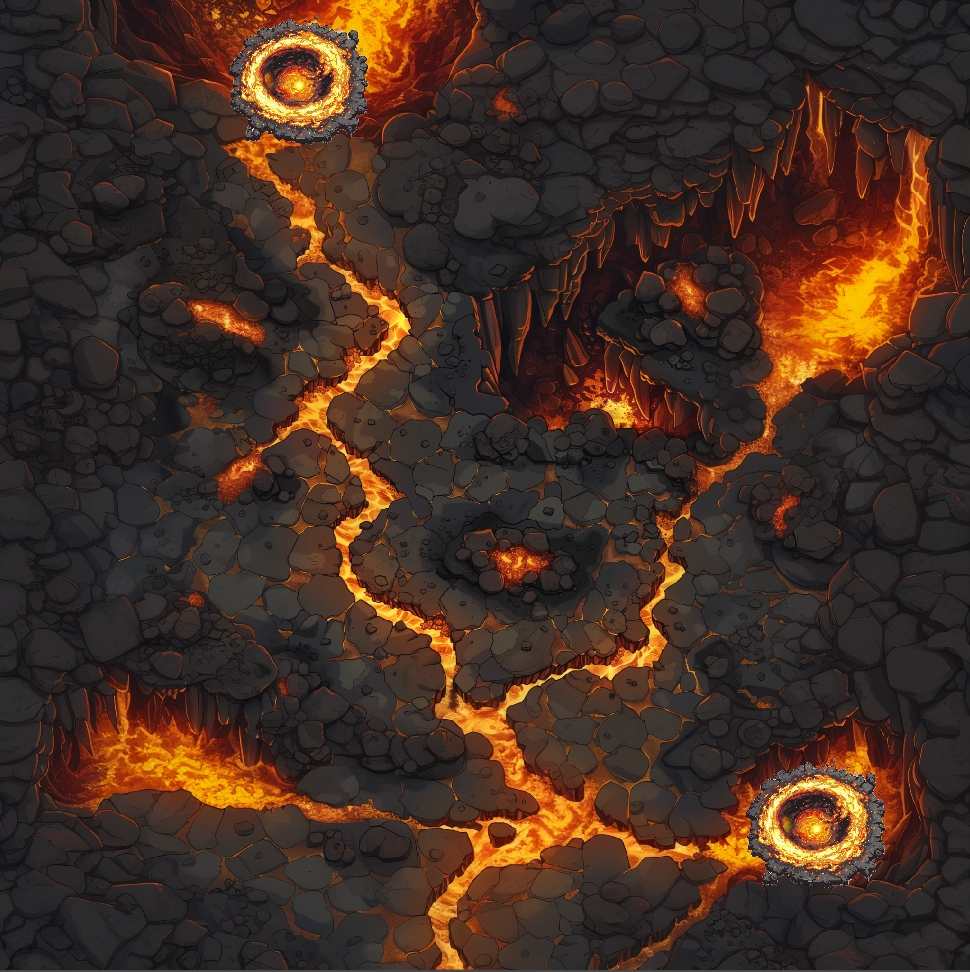
\includegraphics[width=\columnwidth]{figure2.png} % Use the name of your image file
    \caption{Example: Fire Element Zone}
    \label{fig:figure2} % Reference label for the image
\end{figure}
\subsection{Testing and Iteration for Exclusion and Justifications}

\subsubsection{Early Stage Design}
During the early design stage, I focused on eliminating complex and unnecessary mechanics that detracted from the goals of accessibility and real-time immersion. This process involved the exclusion of radial menus, time-stopping skill selection, and complex interactions between spells and enemy elemental properties.
\begin{itemize}
    \item \textbf{Radial Menus:} Though considered as an option for spell selection, radial menus were rejected due to their reliance on time-stopping and precise mouse input. These aspects disrupted the fast-paced flow of combat and complicated input, which contradicted the project’s emphasis on simplicity.
    \item \textbf{Time-Stopping Skill Selection:} Pausing gameplay to choose spells was dismissed as it broke immersion and diminished the urgency of combat. The aim was to provide a seamless, uninterrupted combat experience.
    \item \textbf{Complex Environmental Interactions:} Early concepts included interactions between primary elements and enemy elemental properties. This layer was removed to simplify gameplay, focusing solely on environmental interactions, which offered clearer and more meaningful gameplay feedback.
\end{itemize}

\subsubsection{First Spell-Casting System Design}
The first version of the spell-casting system required players to use multiple buttons (E to open the spell menu, 1-5 to select elements, and Space to confirm and release the spell). This system was tested for speed and accuracy, revealing some initial successes and limitations.
\begin{itemize}
    \item \textbf{Test 1: Speed and Accuracy}
    \begin{itemize}
        \item Players were asked to cast 20 spells, using the system for the first time.
        \item Results showed that after casting 10 spells, players achieved over 90 percent accuracy, with average spell-casting times dropping below 1.5 seconds per spell.
        \item \textbf{Outcome:} While successful in speed and accuracy, the system required extensive left-hand input (7 keys) and overloaded the player, especially during simultaneous aiming with the mouse.
    \end{itemize}
    \item \textbf{Test 2: Environmental Interaction Awareness}
    \begin{itemize}
        \item Players were tested to detect interactions between spells and elemental zones (e.g., primary elements being strengthened or weakened).
        \item Only 20 percent of players noticed these effects in two minutes of gameplay.
        \item \textbf{Solution:} A user interface with pop-up messages and status bar indicators for spell amplification or weakening was implemented. Retesting showed 100 percents awareness after these additions.       
    \end{itemize}
\end{itemize}

\subsubsection{Transition to the Orb-Based System}
Feedback from the first system revealed fundamental issues: over-reliance on the left hand reduced player focus and impaired right-hand precision for aiming. To address these shortcomings, I redesigned the system based on five elemental orbs cycling through highlighted states.

\subsubsection{Second Spell-Casting System Design (Orb-Based)}
The orb-based system allowed players to select elements by pressing Space when the desired orb was highlighted. The system dramatically reduced key inputs while retaining strategic depth.
\begin{itemize}
    \item \textbf{Test 3: Speed and Accuracy with Orb-Based System}
    \begin{itemize}
        \item Five players were tasked with casting 20 specific spells on moving targets.
        \item \textbf{Results:}
        \begin{itemize}
            \item Average spell-casting accuracy reached 95 percents.
            \item Accuracy of hitting moving targets reached 90 percents.
        \end{itemize}
        \item The initial highlight interval was set at 0.5 seconds per orb.
    \end{itemize}
\end{itemize}

\begin{itemize}
    \item \textbf{Test 4: Highlight Interval Adjustment}
    \begin{itemize}
        \item Highlight intervals were tested at 0.3, 0.4, 0.5, 0.6, and 0.7 seconds.
        \item \textbf{Results:}
        \begin{itemize}
            \item At 0.3 seconds: Correct spell selection dropped to 45 percents, and targeting accuracy fell to 60 percents.
            \item At 0.4 seconds: Correct selection rose to 70 percents, with 80 percents targeting accuracy.
            \item At intervals longer than 0.5 seconds, no significant improvement was observed.
        \end{itemize}
        \item \textbf{Conclusion:} A 0.5-second highlight interval offered the optimal balance between speed and accuracy.
    \end{itemize}
\end{itemize}

The iterative design process involved rejecting alternative approaches that failed to meet the project’s goals of simplicity, immersion, and accessibility.

\section{Evaluation Metrics}
To evaluate the effectiveness of the spell-casting system and its impact on real-time combat, this project used a comprehensive set of metrics across three categories: Spell-Casting System Metrics, Real-Time Combat Metrics, and Environmental Interaction Metrics. Additionally, the Variety of Spells Unleashed was measured to assess how well the system enabled diverse spell usage based on the player's tactical needs.

\subsection{Spell-Casting Metrics}
The spell-casting system was evaluated for usability, variety, and responsiveness through the following criteria:

\subsubsection{Ease of Use:}
\begin{itemize}
    \item \textbf{Time Taken to Execute Spells:} Players were timed on how long it took to execute a specific spell using the orb-based system. This metric measured the efficiency of the streamlined input design compared to traditional systems with extensive keybindings.
    \item \textbf{Number of Unique Spells Cast in a Fixed Time:} This metric assessed how effectively players could create and cast multiple spells within a limited period, reflecting the system’s flexibility and player familiarity with the mechanics.
\end{itemize}

\subsubsection{Variety and Responsiveness:}
\begin{itemize}
    \item \textbf{Player Satisfaction with Spell Options:} Qualitative feedback was collected on whether the available elemental combinations met player expectations for variety and strategic depth.
    \item \textbf{Error Rate in Spell Execution:} This metric measured the frequency of incorrect spell selections due to input complexity. A low error rate indicates intuitive design and ease of use.
\end{itemize}

\subsection{Real-Time Combat Metrics}
To assess the effectiveness of the spell-casting system during combat, additional metrics measured player performance and adaptability under pressure:

\subsubsection{Player Dynamic Response to Combat Scenarios:}

\begin{itemize}
    \item \textbf{Adaptability in Combat:} Players were observed for their ability to handle varying enemy behaviors dynamically using the spell system. This included assessing whether players could adjust their spell choices effectively in response to changing conditions.
    \item \textbf{Delay in Casting Spells:} Delays between selecting and executing spells were analyzed to identify bottlenecks in the system that could disrupt combat flow.
\end{itemize}

\subsubsection{Player Comfort with Aiming and Movement:}

\begin{itemize}
    \item \textbf{Accuracy of Targeting Spells:} This metric evaluated how well players could aim and hit moving targets while simultaneously selecting and casting spells. It assessed the balance between cognitive load and real-time decision-making.
    \item \textbf{Integration with Environmental Effects:} Players’ ability to adapt to amplified or weakened spell effects in different elemental zones was tracked, measuring how quickly they recognized and responded to these environmental changes.
\end{itemize}

\subsection{Environmental Interaction Metrics}
The interaction between the player’s spells and the game’s elemental zones was evaluated for impact and player perception:

\subsubsection{Effectiveness of Amplifications and Reductions:}

\begin{itemize}
    \item \textbf{Spell Damage Comparison:} Amplified spell damage was compared to weakened spell damage to ensure that the interactions were noticeable and meaningful without disrupting gameplay balance.
    \item \textbf{Impact Analysis:} Metrics included the percentage difference between amplified and weakened damage, ensuring these effects contributed to strategic depth while remaining intuitive.
\end{itemize}

\subsubsection{Player Feedback on Immersion:}

\begin{itemize}
    \item Players provided qualitative feedback on how intuitive and immersive they found the environmental interactions. This included evaluating visual and auditory cues signaling the effects of environmental zones.
\end{itemize}

\subsection{Variety of Spells Unleashed}
A critical measure of the system’s success was its ability to allow players to unleash a diverse range of spells with minimal keystrokes, tailored to varying combat scenarios. Metrics included:

\subsubsection{Spell Categorization by Primary Element:}
Spells were analyzed based on their primary element:

\begin{itemize}
    \item \textbf{WOOD:} Healing and support.
    \item \textbf{FIRE:} Ranged damage and area attacks.
    \item \textbf{METAL:} High single-target damage.
    \item \textbf{EARTH:} Defensive and shielding abilities.
    \item \textbf{WATER:} Crowd control and sustained damage.
\end{itemize}

\subsubsection{Distribution of Spell Usage:}

\begin{itemize}
    \item The percentage of spells cast across the five primary elements was tracked to assess whether players utilized the full range of spell categories based on combat needs.
    \item Over-reliance on a single element or neglect of others indicated potential design flaws or balance issues.
\end{itemize}

\subsubsection{Adaptation to Combat Scenarios:}
Players were observed for their ability to choose spells aligned with the combat situation. For instance:
\begin{itemize}
    \item Healing spells during critical health states.
    \item High-damage FIRE or METAL spells against strong enemies.
    \item Defensive EARTH spells when overwhelmed by multiple enemies.
\end{itemize}

\subsubsection{Area-Specific Elemental Influences:}
Each Area in the game is themed around a specific element (e.g., Metal, Wood, Water, Fire, Earth). This affects the efficacy of spells cast in that Area based on the interaction between the primary element of the spell and the Area's elemental property:

\begin{itemize}
    \item Spells that align with the Area's element are amplified by 25 percents.
    \item Spells that are restrained by the Area's element are weakened by 25 percents.
    \item Spells with neutral interactions remain unaffected.
    \item \textbf{Impact on Spell Variety:}
    \begin{itemize}
        \item Players were observed to adjust their spell selection dynamically based on the Area they were in. For example:
        \begin{itemize}
            \item In a Water Area, players favored Wood and Fire spells (neutral or amplified effects) while avoiding Metal and Fire spells (weakened effects).
            \item This strategic adaptation ensured that the variety of spells unleashed was not solely dictated by player preference but also by environmental constraints.
        \end{itemize}
    \end{itemize}
\end{itemize}

\subsubsection{Orb-Cycling Time Constraints:}
The elemental orb-cycling system introduces a time-based limitation, as players must wait for the desired orb to be highlighted before selecting it. This constraint influences the composition of spells in real-time combat:

\begin{itemize}
    \item \textbf{Impact on Spell Selection:}
    \begin{itemize}
        \item Spells requiring three identical orbs (e.g., three Fire orbs) inherently take longer to prepare since the player must wait for the same orb to cycle through three times.
        \item Under pressure from fast-approaching enemies, players often opt for faster-to-prepare spells (e.g., spells with three different orbs) over optimal ones with stronger effects.
    \end{itemize}
    \item \textbf{Balancing Design:}
    \begin{itemize}
        \item To incentivize players to endure longer preparation times for spells with identical orbs, these spells are designed to have stronger effects. For example:
        \begin{itemize}
            \item A triple-Fire spell could deal massive area damage with a lingering burn effect.
            \item A triple-Earth spell might provide an unbreakable shield with extended duration.
        \end{itemize}
    \end{itemize}
\end{itemize}

\subsection{Virtualized Test Results: Variety of Spells Unleashed}
To validate the effectiveness of the system, a focused test was conducted with five players tasked to use the orb-based system in a combat simulation. Each player was instructed to handle varied combat scenarios over a 10-minute session, prioritizing adaptability and spell variety. The results were as follows:

\begin{table}[h!]
\centering
\caption{Average Spell Usage by Primary Element}
\label{tab:average-spell-usage}
\resizebox{0.5\textwidth}{!}{%
\begin{tabular}{|c|c|p{3.5cm}|p{3.5cm}|}
\hline
\textbf{Primary Element} & \textbf{Average Spell Usage (\%)} & \textbf{Scenario Examples} & \textbf{Player Feedback} \\ \hline
WOOD & 20\% & Healing teammates; removing debuffs & Players found healing spells critical in survival. \\ \hline
FIRE & 25\% & Attacking large groups of enemies & Fire spells were praised for their visual impact. \\ \hline
METAL & 15\% & Targeting bosses or strong enemies & Effective but limited due to cooldowns. \\ \hline
EARTH & 25\% & Defending against incoming projectiles & Shields provided essential protection under pressure. \\ \hline
WATER & 15\% & Controlling enemy movements & Sustained damage was appreciated in drawn-out fights. \\ \hline
\end{tabular}%
}
\end{table}


\subsubsection{Insights from Testing:}
\begin{itemize}
    \item Players effectively used a variety of spells, with balanced usage across categories except for METAL and WATER, which were situationally dependent.
    \item Adjustments were made to improve the utility of METAL and WATER spells, such as increasing their cooldown efficiency and area of effect.
\end{itemize}

\subsection{Virtualized Test Results: Additional Influences on Spell Variety}
To evaluate the impact of Area-specific elemental effects and orb-cycling constraints on spell variety, a focused test was conducted with five players. Players were tasked with surviving in different elemental Areas for a fixed duration, during which they had to release spells dynamically based on environmental influences and time pressures.

\begin{table}[h!]
\centering
\caption{Preferred Spells by Area}
\label{tab:preferred-spells}
\resizebox{0.5\textwidth}{!}{%
\begin{tabular}{|c|c|p{3.5cm}|p{3.5cm}|c|}
\hline
\textbf{Area} & \textbf{Primary Element} & \textbf{Preferred Spells} & \textbf{Reason for Preference} & \textbf{Percentage of Spells Cast (\%)} \\ \hline
Metal Area & Metal & Fire, Earth & Amplified effects and crowd-control effectiveness. & 60\% \\ \hline
Wood Area & Wood & Fire, Metal & Neutral or amplified effects; avoided Water spells (weakened). & 75\% \\ \hline
Water Area & Water & Wood, Fire & Amplified healing and damage; avoided Earth spells (weakened). & 65\% \\ \hline
Fire Area & Fire & Earth, Water & Defensive or sustained damage to counter high damage dealt by amplified Fire foes. & 70\% \\ \hline
Earth Area & Earth & Metal, Water & Balanced approaches to deal with defensive boosts in Earth Area. & 50\% \\ \hline
\end{tabular}%
}
\end{table}


\subsubsection{Findings:}
\begin{itemize}
    \item Environmental constraints significantly shaped the spells players chose to unleash, ensuring strategic diversity.
    \item Spells with amplified effects in specific Areas were consistently favored, demonstrating the intuitive nature of environmental interactions.
\end{itemize}

Additionally, the impact of the orb-cycling mechanic was evaluated based on player response times and strategic choices during combat:

\begin{table}[h!]
\centering
\caption{Spell Preparation Time vs Effectiveness}
\label{tab:spell-preparation}
\resizebox{0.5\textwidth}{!}{%
\begin{tabular}{|c|c|c|c|}
\hline
\textbf{Spell Type} & \textbf{Preparation Time (Seconds)} & \textbf{Effectiveness} & \textbf{Percentage of Spells Cast (\%)} \\ \hline
Triple-Identical Orbs & Long & Stronger, situational & 20\% \\ \hline
Two Identical + One Orb & Mid & Balanced, versatile & 50\% \\ \hline
Three Different Orbs & Short & Quick, reactive & 30\% \\ \hline
\end{tabular}%
}
\end{table}


\subsubsection{Insights:}
\begin{itemize}
    \item Triple-identical spells were used sparingly but strategically, often reserved for high-stakes scenarios due to their longer preparation time and stronger effects.
    \item Most players relied on faster-to-prepare spells (e.g., three different orbs) for immediate combat needs, highlighting the importance of flexibility in real-time scenarios.
\end{itemize}


\subsection{Why These Metrics?}
The chosen metrics ensured that the system met its design goals of offering accessibility, variety, and strategic depth:
\subsubsection{Time-Based Metrics:}
Validated the system’s responsiveness and usability.
\subsubsection{Categorization Metrics:}
Ensured the spell-casting system provided meaningful choices for diverse combat situations.
\subsubsection{Feedback Metrics:}
Captured subjective user experience and revealed areas for iterative improvement.
\subsubsection{Area-Specific Metrics:}
Highlight how environmental influences dynamically shape player behavior and spell variety.
\subsubsection{Orb-Cycling Metrics:}
Demonstrate the balance between preparation time, spell effectiveness, and player choices under pressure.

\subsection{Excluded Metrics and Justifications}
Alternative metrics, such as in-depth statistical analyses or AI-driven simulations, were considered but excluded:
\subsubsection{Statistical Models:}
Rejected due to the limited scope of player testing and a focus on qualitative feedback.
\subsubsection{AI Simulations:}
While useful, these lacked the human element needed to evaluate usability and player satisfaction.

\section{Results and Discussion}
\subsection{Success of the Spell-Casting System} The spell-casting system successfully addressed the problem of managing diverse combat skills with minimal keyboard input. Testing results revealed that the orb-based system allowed players to dynamically adapt their strategies while maintaining ease of use and responsiveness. Key metrics supporting these findings include:

\subsubsection{Usability and Accessibility} 
\begin{itemize} 
    \item \textbf{Time to Execute Spells:} Players demonstrated an average spell-casting time of 1.2 seconds, a significant improvement over the first version of the spell-casting system, which required multiple keypresses and averaged 2.5 seconds. 
    \item \textbf{Error Rate:} The error rate for incorrect spell execution dropped to 5 percents in the orb-based system compared to 15 percents in earlier iterations. This reduction highlights the intuitive nature of the new system. 
    \item \textbf{Satisfaction Ratings:} Qualitative feedback showed that 90 percents of players rated the orb-based system as intuitive and engaging. Many players specifically appreciated the minimal input requirement and how it freed their left hand for movement while maintaining focus on combat. 
\end{itemize}

\subsubsection{Variety and Strategic Depth} The orb-based system enabled players to unleash a diverse range of spells tailored to combat scenarios: 
\begin{itemize} 
    \item Players effectively utilized spells across all primary elements. For example, healing (WOOD, 20 percents) and area damage (FIRE, 25 percents) spells were frequently used based on tactical needs. 
    \item Spells requiring identical orbs, while used sparingly (20 percents), provided meaningful impact during high-stakes situations, such as boss fights. 
    \item The ability to combine elements dynamically enabled players to create versatile spell chains, reflecting the system’s adaptability. 
\end{itemize}

\subsection{Environmental Interaction Effects} The inclusion of elemental zones significantly enhanced the strategic depth of the game: \begin{itemize} 
    \item \textbf{Amplified and Weakened Effects:} Players quickly adapted to the amplified effects of matching elements (e.g., 25 percents increased damage for FIRE spells in Fire Areas). Conversely, they strategically avoided using weakened spells, highlighting their understanding of environmental mechanics. 
    \item \textbf{Player Feedback:} Players found the interactions intuitive, with 85 percents reporting that the environmental effects added meaningful complexity to gameplay without feeling overwhelming. 
    \item \textbf{Area-Specific Strategies:} The test results showed distinct spell preferences in each Area. For example, in Water Areas, players favored healing and damage spells (Wood and Fire) while avoiding weakened Earth spells. This demonstrated that the environmental interactions dynamically shaped player behavior. 
\end{itemize}

\subsection{Challenges and Iterations} Several challenges arose during development, requiring iterative improvements: 
\begin{itemize} 
    \item \textbf{Input Speed vs. Spell Variety:} Initial tests revealed that faster orb cycles reduced spell accuracy, while slower cycles hindered responsiveness. The finalized 0.5-second interval struck a balance, maintaining both speed and accuracy. 
    \item \textbf{Visual and Auditory Cues:} Early versions of the elemental zones lacked sufficient feedback. Adding glowing cues and auditory signals improved player awareness, with 100 percents of players recognizing environmental effects in retests. 
    \item \textbf{Balancing Spell Effects:} Spells requiring identical orbs initially felt underpowered given their longer preparation times. Increasing their effectiveness (e.g., triple-FIRE causing lingering area burns) incentivized players to endure longer wait times for greater impact. 
\end{itemize}

\subsection{Alternate Explanations} While the metrics indicate the system’s success, alternative factors may have influenced player satisfaction: 
\begin{itemize} 
    \item \textbf{General Game Design:} Positive feedback on the spell-casting system may have been partially influenced by the game’s overall design, including engaging combat scenarios and balanced enemy AI. 
    \item \textbf{Environmental Effects:} Players’ adaptability in elemental zones might also reflect broader environmental design rather than the spell system specifically. 
    \item \textbf{Learning Curve:} Familiarity with the orb system over time may have skewed results, as players became increasingly adept at navigating its mechanics. 
\end{itemize}

\subsection{Impact on Game Design Principles} This project contributes to broader trends in game design by prioritizing accessibility, user experience, and intuitive controls. Key takeaways include: 
\begin{itemize} 
    \item \textbf{Accessible Input Systems:} The orb-based system demonstrates how minimalist controls can offer both depth and flexibility, providing a model for future game designs targeting diverse player demographics. 
    \item \textbf{Strategic Immersion:} By integrating environmental effects and dynamic spell combinations, the project highlights the potential for layered mechanics to enhance engagement without overwhelming players. 
    \item \textbf{Iterative Development:} The success of the system underscores the value of player feedback and iterative testing in refining complex mechanics, a practice that can benefit both indie developers and larger studios. 
\end{itemize}

\subsection{Remaining Limitations} Despite its successes, the system has some limitations: 
\begin{itemize} 
    \item \textbf{Overpowered Combinations:} Certain spells (e.g., triple-FIRE) may still feel overpowered in specific scenarios, requiring further balancing. 
    \item \textbf{Reliance on Visual Cues:} Players with visual impairments may struggle with the system, highlighting the need for additional accessibility features such as tactile or auditory feedback. 
    \item \textbf{Limited Enemy Interactions:} While environmental effects were well-received, the removal of direct interactions between spells and enemy elements may have reduced strategic complexity in combat. \end{itemize}

\section{Ethical Considerations}
The development of this project raises several ethical considerations, including accessibility, potential bias in game design, the broader impact on equity within the gaming community, and the use of AI-generated assets.

\subsection{Accessibility and Inclusivity} The spell-casting system emphasizes accessibility by reducing reliance on complex input mechanics. However, the reliance on visual cues, such as the orb-highlighting mechanism, could pose challenges for players with visual impairments. Future iterations of the system should integrate alternative feedback mechanisms, such as auditory or tactile cues, ensuring a more inclusive experience.

\subsection{Bias in Game Design} Bias can inadvertently influence game mechanics and aesthetics. For example, associating certain elemental properties (e.g., Fire for destruction, Water for control) with specific cultural or philosophical interpretations risks perpetuating stereotypes. By adopting the Wu Xing system, rooted in Chinese philosophy, this project recognizes its cultural significance but strives to maintain neutrality in its application, ensuring that these mechanics remain universally applicable and respectful.

\subsection{Equity and Societal Impact} As gaming becomes increasingly diverse, it is critical to consider the global audience. This project’s focus on accessibility aligns with broader trends in making games playable across a wide demographic spectrum, including individuals who may lack advanced gaming hardware or have limited physical mobility. However, the potential inequity in access to educational resources for learning such complex systems, such as coding and game development, highlights the need for freely available tutorials and documentation to democratize game development.

\subsection{Future Contributions} This project’s emphasis on accessible game mechanics and skill diversity serves as a template for broader industry adoption, contributing to reducing barriers in gaming. It demonstrates how broadening the range of skills players can choose from during a matchup adds depth, complexity, and enjoyment to the game. Such innovations not only enrich gameplay but also offer valuable insights into designing games that cater to a wide variety of player preferences and abilities.

\subsection{Concerns Regarding AI-Generated Assets} One potential concern with this project is the reliance on AI-generated assets. Some assets, such as textures or models, were generated using AI mapping tools. While these tools can significantly reduce development time, they raise ethical questions about originality, copyright, and the potential displacement of human artists. Developers using similar methods should carefully consider licensing terms and seek to balance AI use with creative, human-generated contributions.

\section{Replication Instrcutions}
\subsection{Required Software and Tools} To replicate this project, the following software and tools are required: 
\begin{itemize} 
    \item Unity Game Engine: Version 2022.3.49f1 (LTS). Download from \url{https://unity.com}. 
    \item A Pathfinding Project*: Version 4.2.17, available at \url{https://arongranberg.com/astar/}. 
    \item C\#.NET Framework: Ensure compatibility with Unity’s default scripting environment. 
    \item Visual Studio 2022: Recommended IDE for scripting, available at \url{https://visualstudio.microsoft.com}. 
    \item 2D Assets: Placeholder assets can be sourced from \url{https://itch.io} or generated using AI tools such as MidJourney combined with Photoshop for refinement. 
    \item Git: For version control. 
\end{itemize}

\subsection{Setup Instructions}
\begin{enumerate}
    \item \textbf{Install Unity:} Install version 2022.3.49f1 (LTS) and create a new 2D project.
    \item \textbf{Add A* Pathfinding Package:}
    \begin{itemize}
        \item Download and import version 4.2.17 of the package into the Unity project.
        \item Configure the A* Pathfinding system according to the provided scripts.
    \end{itemize}
    \item \textbf{Import Scripts:}
    \begin{itemize}
        \item Place the provided scripts (available in the project repository) into the \texttt{Assets/Scripts} directory.
        \item Ensure all dependencies are correctly resolved in Unity’s Inspector.
    \end{itemize}
    \item \textbf{Test the Game:}
    \begin{itemize}
        \item Open the sample scene included in the repository.
        \item Test the spell-casting system by pressing \texttt{Play} and experimenting with the elemental orb mechanics.
    \end{itemize}
\end{enumerate}

\subsection{Asset Sourcing} Developers can source free 2D assets from platforms like \url{https://itch.io}, which offers a wide range of free and paid game assets. Alternatively, AI-driven tools such as MidJourney can generate unique assets. These assets can then be refined using tools like Photoshop to ensure they fit the game’s aesthetic and gameplay requirements. Developers must ensure that any AI-generated assets comply with licensing and copyright laws.

\subsection{Dependencies and Compatibility** Ensure all software versions match the specified requirements. Future users are advised to update Unity LTS versions only after verifying compatibility with A* Pathfinding and project scripts.}\

\appendix
\section{Code Architecture Overview}

This appendix outlines the organization of the code, explaining the purpose of each script, how it is attached to GameObjects in Unity, and its role in the project. The code structure has been designed with modularity and scalability in mind, making it easier for other developers to extend or debug.

\subsection{Hierarchy and Code Breakdown}

\subsubsection{1. \texttt{GameManager}}
\begin{itemize}
    \item \textbf{Purpose}: Initializes the game by deactivating all areas, including their enemy spawners, A* pathfinding graphs, and environments. It then places the player on a random entry portal and activates the corresponding area.
    \item \textbf{Scripts Attached}:
    \begin{itemize}
        \item \texttt{GameManager}:
        \begin{itemize}
            \item Turns off all elements of the game world during initialization.
            \item Places the player in a random entry portal.
            \item Activates the appropriate area based on the portal.
        \end{itemize}
    \end{itemize}
    \item \textbf{Justification}: Centralized initialization logic ensures all game components start in a predictable state, simplifying debugging and providing flexibility for expansion.
\end{itemize}

\begin{figure}[h]
    \centering
    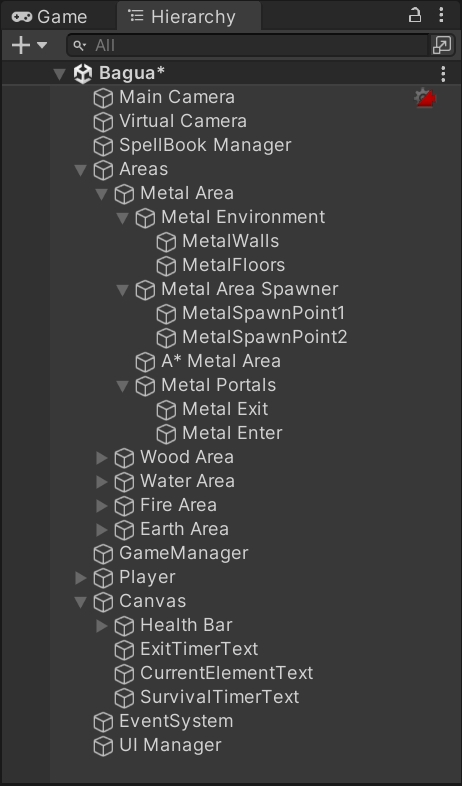
\includegraphics[width=\columnwidth]{figure3.png} % Use the name of your image file
    \caption{Hierarchy in Unity}
    \label{fig:figure3} % Reference label for the image
\end{figure}

\subsubsection{2. \texttt{Areas (e.g., Metal Area, Wood Area)}}
\begin{itemize}
    \item \textbf{Purpose}: Represents distinct areas of the game world with unique environmental properties, enemies, and mechanics.
    \item \textbf{Components}:
    \begin{itemize}
        \item \textbf{Environment} (e.g., \texttt{MetalWalls}, \texttt{MetalFloors}):
        \begin{itemize}
            \item Contains the visual and physical elements of the area.
            \item Includes a \texttt{Polygon Collider} to define the camera bounds for the area.
        \end{itemize}
        \item \textbf{A* Pathfinding Graph}:
        \begin{itemize}
            \item Manages enemy pathfinding within the area.
            \item Deactivated when the area is not active to save memory.
        \end{itemize}
        \item \textbf{Portals}:
        \begin{itemize}
            \item Handle transitions between areas.
        \end{itemize}
    \end{itemize}
    \item \textbf{Scripts Attached}:
    \begin{itemize}
        \item \texttt{AreaManager}:
        \begin{itemize}
            \item Activates and deactivates the environment, enemy spawners, and A* pathfinding graph.
            \item Tracks the area's main element for interaction with spells.
        \end{itemize}
        \item \texttt{EnemySpawner}:
        \begin{itemize}
            \item Spawns different types of enemies dynamically at predefined points.
            \item Mounted with multiple enemy prefabs for random generation.
        \end{itemize}
        \item \texttt{PortalSystem}:
        \begin{itemize}
            \item Manages transitions between areas by deactivating the current area and activating the target area.
            \item Turns off enemy spawners, destroys remaining enemies, deactivates the tilemap to save memory, and turns off the A* pathfinding graph in the current area.
            \item Activates the target area and scans the grid graph for enemies in the new area.
        \end{itemize}
    \end{itemize}
    \item \textbf{Justification}:
    \begin{itemize}
        \item Modularity for individual areas allows scalable development.
        \item The \texttt{PortalSystem} acts as a secondary game manager to handle area transitions seamlessly.
    \end{itemize}
\end{itemize}

\subsubsection{3. \texttt{Player}}
\begin{itemize}
    \item \textbf{Purpose}: Represents the player character, handling movement, health, and interactions.
    \item \textbf{Components}:
    \begin{itemize}
        \item \textbf{Element Balls}: Child objects attached to the player. These work with the \texttt{ElementSelector} script to handle element selection for spellcasting.
    \end{itemize}
    \item \textbf{Scripts Attached}:
    \begin{itemize}
        \item \texttt{PlayerController}:
        \begin{itemize}
            \item Manages player movement, health, and invincibility logic.
            \item Handles collisions with enemies to take damage.
        \end{itemize}
        \item \texttt{ElementSelector}:
        \begin{itemize}
            \item Handles the logic for selecting elements and casting spells.
            \item Integrates with the \texttt{SpellBook} to fetch and instantiate the correct spell prefab.
        \end{itemize}
        \item \texttt{ElementBall}:
        \begin{itemize}
            \item Displays available elements for selection and highlights the currently active selection.
        \end{itemize}
    \end{itemize}
    \item \textbf{Justification}:
    \begin{itemize}
        \item Clear separation of movement, health, and spellcasting simplifies future extensions.
        \item Element selection mechanics are isolated, making it easier to add new elements or modify the system.
    \end{itemize}
\end{itemize}

\subsubsection{4. \texttt{Canvas (UI)}}
\begin{itemize}
    \item \textbf{Purpose}: Displays player health, exit portal timer, survival time, and the current area's element.
    \item \textbf{Components}:
    \begin{itemize}
        \item \textbf{Health Bar}: Visualizes the player's current health.
        \item \textbf{ExitTimerText}: Shows the remaining time until the exit portal unlocks.
        \item \textbf{CurrentElementText}: Displays the active element of the area.
        \item \textbf{SurvivalTimerText}: Tracks how long the player has survived.
    \end{itemize}
    \item \textbf{Scripts Attached}:
    \begin{itemize}
        \item \texttt{UIManager}:
        \begin{itemize}
            \item Updates UI elements dynamically based on game events.
        \end{itemize}
    \end{itemize}
    \item \textbf{Justification}:
    \begin{itemize}
        \item A centralized UI system simplifies the addition of new UI features.
    \end{itemize}
\end{itemize}

\subsubsection{5. \texttt{Enemy}}
\begin{itemize}
    \item \textbf{Purpose}: Represents enemy behavior and interaction with the player.
    \item \textbf{Components}:
    \begin{itemize}
        \item \textbf{A* Pathfinding Scripts}:
        \begin{itemize}
            \item \texttt{Seeker}: Calculates paths for the enemy to reach the target.
            \item \texttt{AIPath}: Handles the movement logic for following the path.
            \item \texttt{AIDestinationSetter}: Sets the player as the target for the enemy.
        \end{itemize}
        \item \textbf{Custom Enemy Scripts}:
        \begin{itemize}
            \item \texttt{EnemyController}:
            \begin{itemize}
                \item Manages enemy health, knockback, and death logic.
            \end{itemize}
            \item \texttt{EnemyTargetAssigner}:
            \begin{itemize}
                \item Hooks the player to the \texttt{AIDestinationSetter}'s target dynamically.
            \end{itemize}
            \item \texttt{NormalEnemy}, \texttt{SelfExplodedEnemy}, \texttt{RushEnemy}:
            \begin{itemize}
                \item Extend the base \texttt{EnemyController} to add unique behaviors for each enemy type.
            \end{itemize}
        \end{itemize}
    \end{itemize}
\end{itemize}

\subsubsection{6. \texttt{Weapon (Spells)}}
\begin{itemize}
    \item \textbf{Purpose}: Handles spellcasting and projectile-based damage dealing.
    \item \textbf{Components}:
    \begin{itemize}
        \item \texttt{SpellBook}:
        \begin{itemize}
            \item Stores all created spells, including their:
            \begin{itemize}
                \item \textbf{Fancy Name}: A readable name for the player.
                \item \textbf{Spell Name}: A key that matches the player's selected elements.
                \item \textbf{Main Element}: Used to interact with the area's element for damage bonuses or penalties.
            \end{itemize}
        \end{itemize}
    \end{itemize}
\end{itemize}

\textbf{This structure ensures modular development and extensibility, making it easier for other developers to debug or enhance specific components.}

\begin{figure}[h]
    \centering
    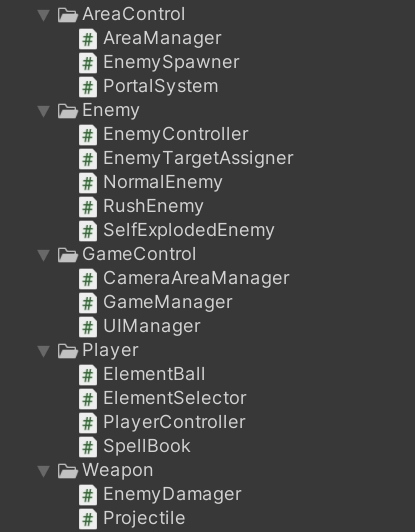
\includegraphics[width=\columnwidth]{figure4.png} % Use the name of your image file
    \caption{Code Structure}
    \label{fig:figure4} % Reference label for the image
\end{figure}

\end{document}
